% vim: spelllang=es

\chapter{Entendiendo Tremor}\label{ch:tremor}

\section{Procesado de Eventos}

Tremor es un \emph{Sistema de Procesado de Eventos}, que consiste en ``el
monitorizado y análisis (procesado) de flujos de información (datos) sobre cosas
que pasan (eventos)''~\cite{luckham2011event}. Tremor fue creado como una
alternativa de alto rendimiento a herramientas como \textcite{logstash} o
\textcite{telegraf}, pero ha evolucionado para soportar casos de uso más
complejos. Al contrario que esos programas, Tremor también tiene soporte para
\emph{agregación} y \emph{rollups}, e incluye un lenguaje \emph{ad hoc} para
\emph{Extract, Transform, and Load} (ETL).

% TODO: hace falta esto?
\textcite{robins2010complex} y \textcite{cugola2012processing} introducen en
detalle los dos campos contenidos en Procesado de Eventos: \emph{Procesado de
Eventos Complejos} y \emph{Procesado de Flujos de
Eventos}\footnote{\emph{Complex Event Processing} y \emph{Event Stream
Processing} respectivamente, siguiendo la terminología anglosajona.}, ambos
relevantes a Tremor. \textcite{dayarathna2018recent} y
\textcite{tawsif2018review} resumen los avances más recientes en el campo,
analizan su evolución, y clasifican sus subáreas. La mayoría de la información
teórica en esta sección se extrae de estas fuentes.

\section{Casos de uso}

La Figura~\ref{fig:tremor_example} ilustra uno de los casos de uso más básicos
de Tremor:

\begin{enumerate}
    \item Recibir \emph{logs} (eventos) de aplicaciones en diferentes protocolos
        o formatos. Es posible que esta heterogeneidad se deba a que algunas
        aplicaciones son legadas y no se puedan reducir a un único protocolo o
        formato, o que esta tarea es demasiado compleja como para gestionarse a
        nivel de aplicación.

    \item Filtrar los eventos redundantes, añadir campos nuevos o eliminar
        aquellos innecesarios y transformar todo a un mismo formato. El uso de
        una herramienta ineficiente o \emph{ad hoc} por la empresa podría ser
        inviable dada una cantidad de datos suficientemente grande o demasiados
        protocolos y formatos como para implementarlos todos.

    \item Enviar todos los logs estructurados a una base de datos para
        analizarlos posteriormente.

\end{enumerate}

\begin{figure}
    \centering
    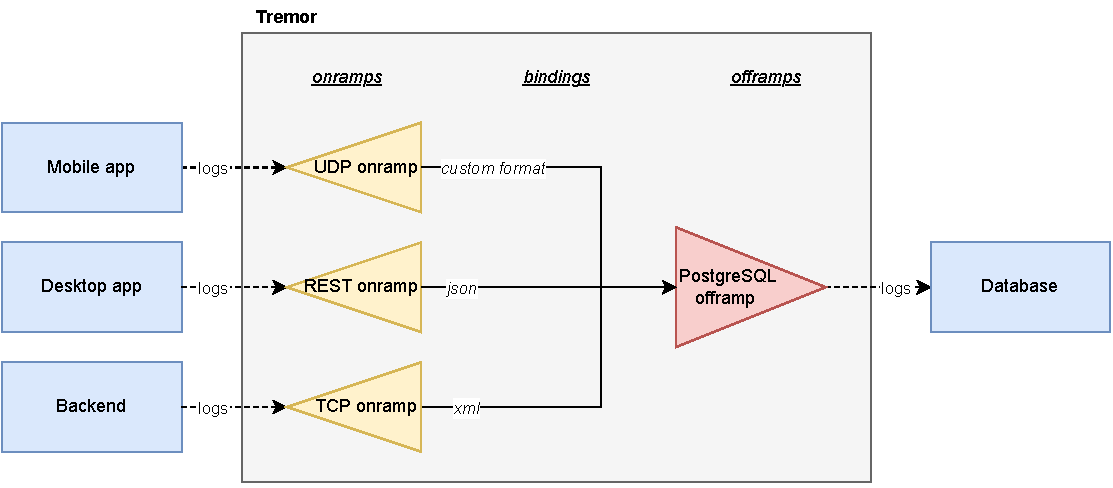
\includegraphics[width=\textwidth]{./Imagenes/example.pdf}
    \caption{Ejemplo de uso básico de Tremor}%
    \label{fig:tremor_example}
\end{figure}

Sin embargo, este caso subestima el potencial de Tremor. La entrada y salida del
sistema se pueden abstraer más, por ejemplo implementando un chatbot que
reproduce música. Este podría tomar mensajes de Discord como su entrada, y
enviar comandos con el API de Spotify como salida.

\section{Conceptos básicos}

Tremor se basa en los términos de \onramps o \sources y \offramps o \sinks:

\begin{itemize}
    \item Una \onramp especifica cómo Tremor se conecta con el mundo exterior (o
        una \pipeline) para \textbf{recibir} de sistemas externos. Por ejemplo
        TCP, periódicamente o PostgreSQL~\cite{tremoronramps}.

    \item Una \offramp especifica cómo Tremor se conecta con el mundo exterior
        (o una \pipeline) para \textbf{enviar} a sistemas externos. Por ejemplo,
        \emph{stdout}, Kafka o ElasticSearch~\cite{tremorofframps}.

    \item Una \pipeline es una lista de operaciones (transformación, agregación,
        eliminación, etc) a través de la cual se pueden encaminar los
        eventos~\cite{tremorpipelines}. La Figura \ref{fig:tremor_pipeline}
        muestra un ejemplo de una \pipeline, definida con Troy, su propio
        lenguaje inspirado en SQL.

\end{itemize}

\begin{figure}
    \centering
    \begin{minted}[escapeinside=||]{mysql}
|\textcolor{blue}{define pipeline}| main
# The exit port is not a default port, so we have to overwrite the
# built-in port selection
into |out, exit|
|\textcolor{blue}{pipeline}|
  # Use the `std::string` module
  use std::|string|;
  use lib::scripts;

  # Create our script
  create |\textcolor{blue}{script}| punctuate from scripts::punctuate;

  # Filter any event that just is `"exit"` and send it to the exit port
  select {"graceful": false} from |in| where event == "exit" into |exit|;

  # Wire our capitailized text to the script
  select |string|::capitalize(event) from |in| where event != "exit"
    into punctuate;
  # Wire our script to the output
  select event from punctuate into |out|;
end;
    \end{minted}
    \caption{Ejemplo de una \pipeline definida para Tremor}%
    \label{fig:tremor_pipeline}
\end{figure}

Estos \onramps u \offramps suelen contener una cantidad de información que es
demasiado grande como para guardarla y debería tratarse en tiempo real. Su
procesado se basa en las siguientes operaciones:

\begin{itemize}
    \item \emph{Filtros}: descarte de eventos completos a partir de reglas
        configuradas, con el objetivo de eliminar información de la \pipeline
        que no se considera relevante.

    \item \emph{Transformaciones}: conversión de los datos de un formato a otro,
        así como incrementar un campo con un contador, reemplazar valores, o
        reorganizar su estructura.

    \item \emph{Matching}: búsqueda de partes de los eventos que siguen un
        patrón en específico (e.g., un campo \code{"id"} con un valor númerico)
        para transformarlo o descartarlo.

    \item \emph{Agregación} o \emph{rollups}: recolección de múltiples eventos
        para producir otros nuevos (e.g., la media o máximo de un campo), de
        forma que la información útil se reduzca en tamaño.

\end{itemize}

Finalmente, otros términos misceláneos sobre Tremor:

\begin{itemize}
    \item \emph{Códec}: describen cómo decodificar los datos del flujo y como
        volverlos a codificar. Por ejemplo, si los eventos de entrada usan JSON,
        tendrá que especificarse ese códec para que lo pueda entender Tremor.

    \item \emph{Preprocesador} o \emph{postprocesador}: operadores sobre flujos
        de datos brutos. Un preprocesador aplicará esta operación antes del
        códec y un postprocesador después. Por ejemplo, \code{base64} codifica o
        decodifica la información con ese protocolo.

    \item \emph{Artefacto}: término genérico para hablar de \sinks, \sources,
        códecs, preprocesadores y postprocesadores.

\end{itemize}

% TODO: explain 'artefacts', 'pre/postprocessors', 'codecs', 'operators'

Para más información sobre Tremor se puede consultar \textcite{tremorintro}, que
introduce sus conceptos más básicos y sus posibles usos --- o cuándo \emph{no}
usarlo, en \textcite{tremorconstraints}. \textcite{tremorrecipes} lista un total
de 32 ejemplos de cómo configurar y emplear el software.

\section{Conectores}

Sin embargo, es posible que algunas \onramps no solo quieran recibir de sistemas
externos, sino también responderles directamente, actuando como una \offramp y
viceversa. Esto es especialmente útil para casos como REST y \websockets, donde
el protocolo da la posibilidad de responder a eventos, por ejemplo con un ACK,
usando la misma conexión. En la versión 0.11 --- la presente cuando me uní al
proyecto --- este problema se solucionaba con el concepto de \emph{linked
transports}.

El término \emph{conector} se introdujo en mayo de 2022 con la versión 0.12.
Solucionan el problema desde el inicio, abstrayendo tanto los \onramps como los
\offramps bajo el mismo concepto, incluyendo los \emph{linked transports}. Dado
que estos ya estaban siendo desarrollados mientras 0.11 era la última versión,
el sistema de plugins se enfocó a conectores desde el principio, en lugar de
\onramps u \offramps, que actualmente están en desuso.

A nivel de implementación, los conectores se definen con el \trait
\code{Connector}, incluido en la figura \ref{fig:tremor_connector_trait}.
Esencialmente, los plugins de tipo conector exportarán públicamente esta
interfaz en su binario, y la runtime deberá ser capaz de cargarlo dinámicamente.
Actualmente, todos los conectores disponibles se listan y cargan de forma
estática al inicio del programa.

\begin{figure}[h]
    \centering
    \begin{minted}{rust}
pub trait Connector {
    /// Crea la parte "source" del conector, si es aplicable.
    async fn create_source(
        &mut self,
        _source_context: SourceContext,
        _builder: source::SourceManagerBuilder,
    ) -> Result<Option<source::SourceAddr>> {
        Ok(None)
    }

    /// Crea la parte "sink" del conector, si es aplicable.
    async fn create_sink(
        &mut self,
        _sink_context: SinkContext,
        _builder: sink::SinkManagerBuilder,
    ) -> Result<Option<sink::SinkAddr>> {
        Ok(None)
    }

    /// Intenta conectarse con el mundo exterior. Por ejemplo, inicia la
    /// conexión con una base de datos.
    async fn connect(
        &mut self,
        _c: &ConnectorContext,
        _attempt: &Attempt
    ) -> Result<bool> {
        Ok(true)
    }

    /// Llamado una vez cuando el conector inicia.
    async fn on_start(&mut self, _c: &ConnectorContext) -> Result<()> {
        Ok(())
    }
    /// Llamado cuando el conector pausa.
    async fn on_pause(&mut self, _c: &ConnectorContext) -> Result<()> {
        Ok(())
    }
    /// Llamado cuando el conector continúa.
    async fn on_resume(&mut self, _c: &ConnectorContext) -> Result<()> {
        Ok(())
    }
    /// Llamado ante un evento de "drain", que se asegura de que no
    /// lleguen más eventos a este conector.
    async fn on_drain(&mut self, _c: &ConnectorContext) -> Result<()> {
        Ok(())
    }
    /// Llamado cuando el conector para.
    async fn on_stop(&mut self, _c: &ConnectorContext) -> Result<()> {
        Ok(())
    }
}
    \end{minted}
    \caption{Simplificación del \trait \code{Connector}}%
    \label{fig:tremor_connector_trait}
\end{figure}

Por tanto, es importante mantener la interfaz de plugins lo más simple posible.
Los detalles de comunicación deberían dejarse a la runtime, de forma que los
plugins se limiten a exportar una lista de funciones síncronas. De esta forma,
se podrá evitar pasar tipos complejos (\code{async}, canales de comunicación,
etc) entre la runtime y los plugins, que implicaría una carga de trabajo mucho
más alta.

Una vez esta interfaz de bajo nivel se defina, se puede crear un \emph{wrapper}
de más alto nivel en la runtime que se encargue de la comunicación y de mejorar
su usabilidad dentro de Tremor. Esto mismo lo hacen otras \crates como
\cratelink{rdkafka}, que implementa una capa de abstracción asíncrona sobre su
interfaz de C en \cratelink{rdkafka-sys}.

\section{Arquitectura interna}

Antes de comenzar a modificar el código existente en Tremor, es importante
conocer cómo funciona para evitar perder el tiempo. Tremor se basa en el modelo
actor. Citando Wikipedia:

% TODO: puedo hacer estas cosas? Me faltaría poner una citación a
% https://en.wikipedia.org/wiki/Actor_model al final del quote, pero así me
% ahorro explicarlo yo mismo.
``[The actor model treats the] actor as the universal primitive of concurrent
computation. In response to a message it receives, an actor can: make local
decisions, create more actors, send more messages, and determine how to respond
to the next message received. Actors may modify their own private state, but can
only affect each other indirectly through messaging (removing the need for
lock-based synchronization).''

No usa un lenguaje (e.g., Erlang) o framework (e.g., \cratelink{bastion}, quizá
en el futuro) que siga estrictamente este modelo, pero re-implementa los mismos
patrones frecuentemente de forma manual. Tremor se basa en \emph{programación
asíncrona}, es decir, que en vez de hilos trabaja con \emph{tareas}, un concepto
de nivel más alto y especializado para entrada/salida. De la documentación de
\cratelink{async-std}, la runtime asíncrona que usa Tremor:

% TODO: faltaría referenciar
% https://docs.rs/async-std/1.10.0/async_std/task/index.html
``An executing asynchronous Rust program consists of a collection of native OS
threads, on top of which multiple stackless coroutines are multiplexed. We refer
to these as “tasks”. Tasks can be named, and provide some built-in support for
synchronization.''

Podríamos resumir su arquitectura con la frase ``Tremor se basa en actores
corriendo en tareas diferentes, que se comunican asíncronamente con canales''.

\section{Detalles de implementación}

El actor principal se llama \code{World}. Contiene el estado del programa, como
los artefactos disponibles (\emph{repositorios}) y los que se están ejecutando
(\emph{registros}) y se usa para inicializar y controlar el programa.

Los \emph{managers} o \emph{gestores} son simplemente actores en el sistema que
envuelven una funcionalidad. Ayudan a desacoplar la comunicación y la
implementación de la funcionalidad interna. De esta forma, se puede eliminar
código repetitivo al inicializar los componentes, así como la creación de
canales de comunicación o el lanzamiento del componente en una tarea nueva.
Generalmente, hay un gestor por cada tipo de artefacto para facilitar su
inicialización y también uno por cada instancia que se esté ejecutando, para
controlar su comunicación.

Notar que la inicialización de los conectores ocurre en dos pasos. Primero se
\emph{registran}, es decir, se indica su disponibilidad para cargarlo
(añadiéndolo al repositorio). Posteriormente, no se ejecutará hasta conectarse
con otro artefacto con \code{launch_binding}, lo cual lo movería del repositorio
al registro, junto al resto de artefactos ejecutándose.

\subsection{Registro}

La Figura~\ref{fig:tremor_registering} detalla todos los pasos seguidos en el
código. Primero han de inicializarse los gestores, y después registrar los
artefactos. Actualmente, esta parte se realiza de forma estática con
\code{register_builtin_types}, pero después de implementar el PDK, debería ser
dinámicamente. Tremor buscaría automáticamente plugins en sus directorios
configurados e intentaría registrar todos los que encuentre. En una futura
versión, el usuario podría solicitar manualmente el cargado de un plugin nuevo
mientras se está ejecutando Tremor.

\begin{figure}
    \centering
    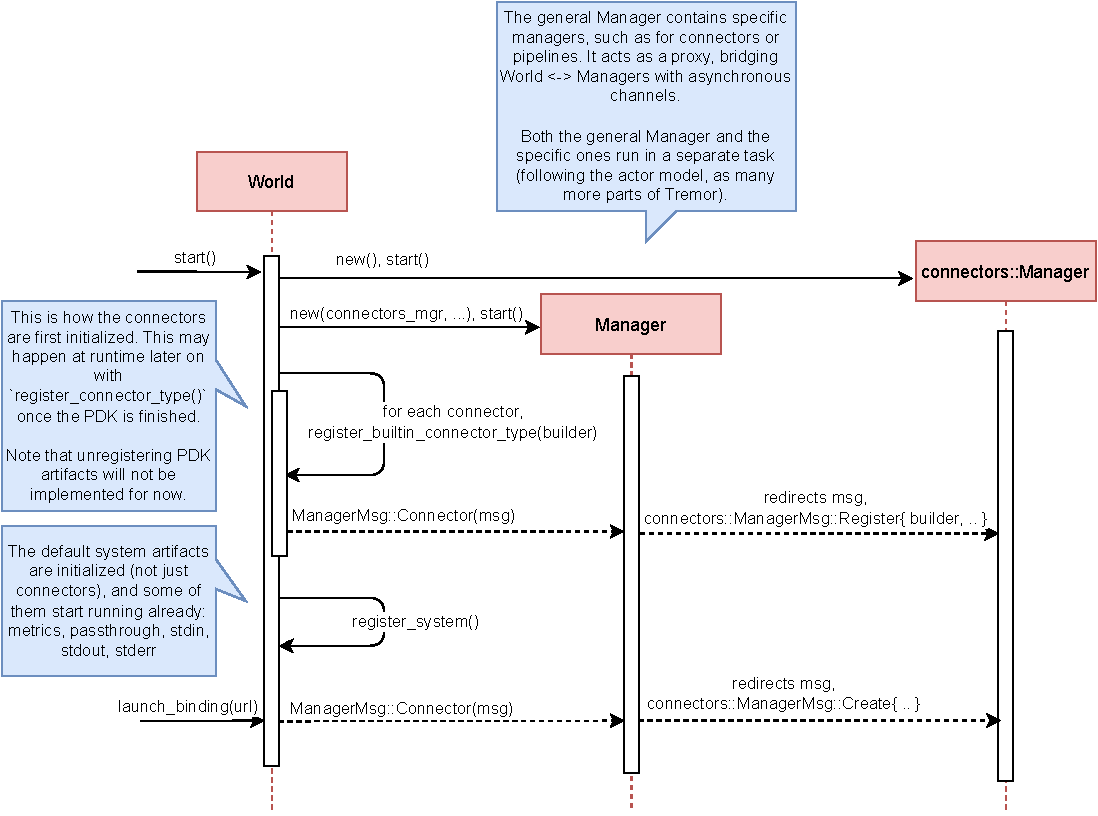
\includegraphics[width=\textwidth]{./Imagenes/registering.pdf}
    \caption{Registro de un conector en el programa}%
    \label{fig:tremor_registering}
\end{figure}

\subsection{Inicialización}

Ya que es un proceso en múltiples pasos (en la implementación es más complicado
que registro + creación), la primera parte provee las herramientas para
inicializar el conector (el \emph{builder}). Cuando el conector necesite
comenzar a ejecutarse porque se haya añadido a una \pipeline, el \builder ayuda
a construir y configurarlo de forma genérica. Finalmente, se añade a una tarea
propia para que se pueda comunicar con otras partes de Tremor. El gestor
\code{connectors::Manager} contiene todos los conectores ejecutándose en Tremor,
como se muestra en la Figura~\ref{fig:tremor_initializing}.

\begin{figure}
    \centering
    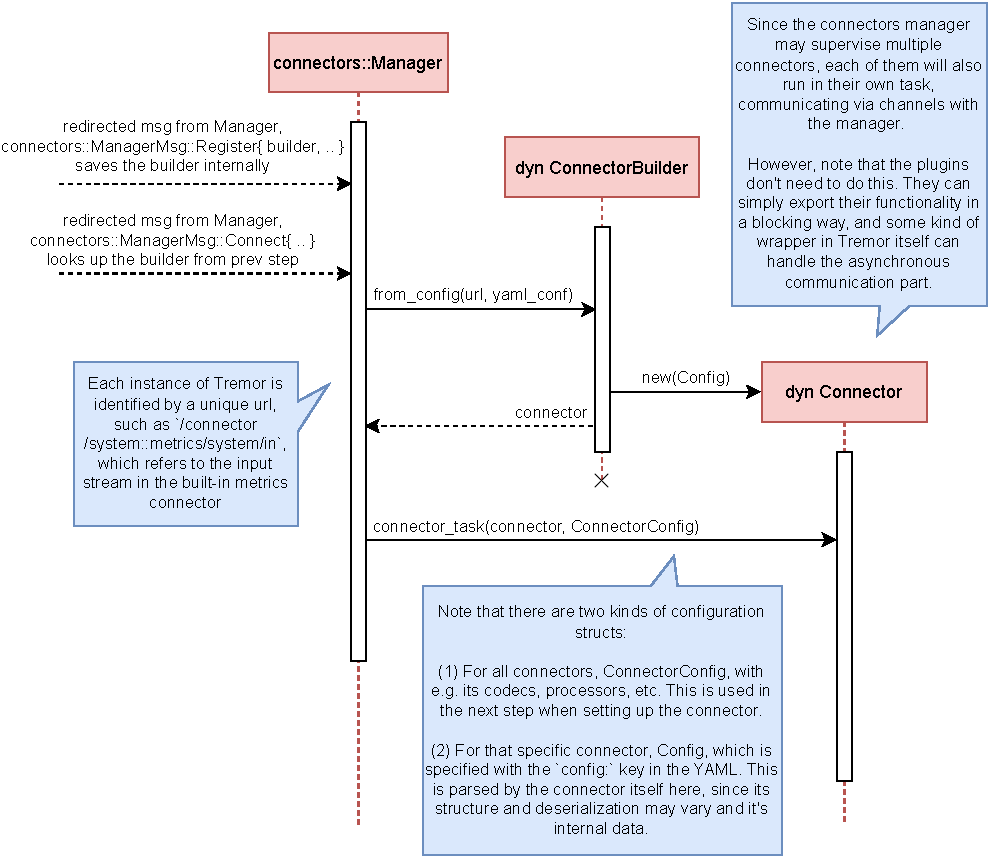
\includegraphics[width=\textwidth]{./Imagenes/initializing.pdf}
    \caption{Inicialización de un conector en el programa}%
    \label{fig:tremor_initializing}
\end{figure}

\subsection{Configuración}

Una vez haya un conector corriendo, la Figura \ref{fig:tremor_setting_up}
visualiza cómo se divide en una parte \sink y otra \source. Estas son
opcionales, pero no exclusivas, así que se puede tener cualquiera de las dos o
ambas. De forma similar, un \builder se usa para inicializar las partes y a
continuación inicia una nueva tarea para ellos.

\begin{figure}
    \centering
    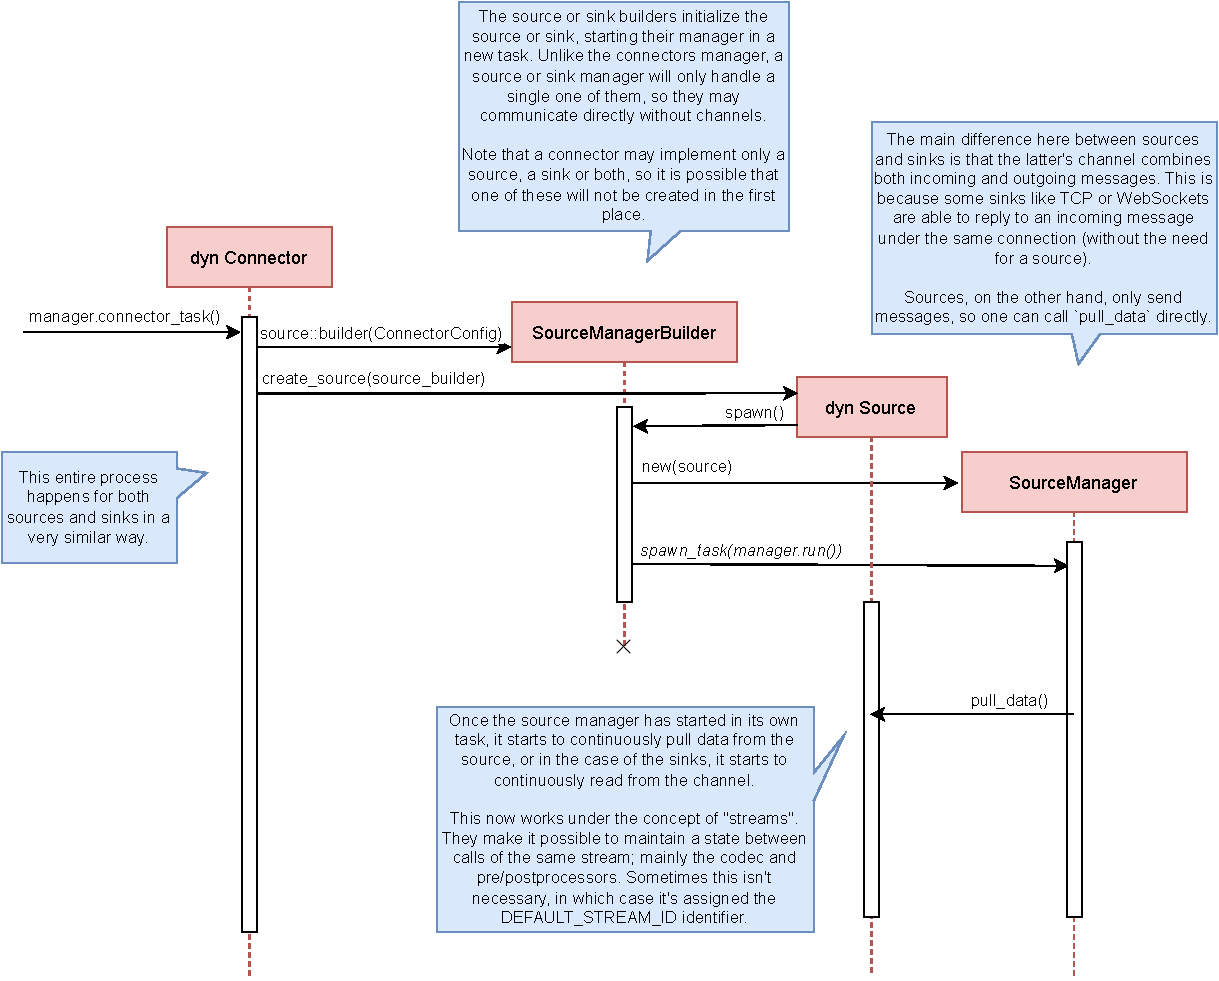
\includegraphics[width=\textwidth]{./Imagenes/setting-up.pdf}
    \caption{Configuración de un conector en el programa}%
    \label{fig:tremor_setting_up}
\end{figure}

También se crea un gestor por cada instancia de \sink o \source, que se
encargará de la comunicación con otros actores. De esta forma, sus interfaces
pueden mantenerse lo más simple posible. Esos gestores recibirán peticiones de
conexión de la \pipeline y posteriormente leerán o enviarán eventos en ella.

La diferencia principal entre \sources y \sinks a nivel de implementación es que
este último también puede responder a mensajes usando la misma conexión. Esto es
útil para notificar que el paquete ha llegado (\code{Ack}) o que algo ha fallado
(\code{Fail} para un evento específico, \code{CircuitBreaker} para dejar de
recibir datos por completo).

Los códecs y preprocesadores se involucran aquí tanto para los \sources como
para los \sinks. En la parte de \source, los datos son transformados a través de
una cadena de preprocesadores y posteriormente se aplica un códec. Para los
\sinks, se sigue el proceso inverso: los datos se codifican primero a bytes con
el códec, y posteriormente una serie de postprocesadores se aplican a los datos
binarios.

\subsection{Notas adicionales}

Algunos conectores se basan en \emph{flujos}. Son equivalentes a los flujos de
TCP, que ayudan a agrupar mensajes para evitar mezclarlos. Se inician y
finalizan mediante mensajes, y el gestor se guarda el estado del flujo en un
campo llamado \code{states} (ya que, por ejemplo, algunos preprocesadores puedan
querer guardar un estado). Si un conector no necesita flujos, como
\code{metronome} (que únicamente envía eventos periódicamente), puede
especificar su identificador de flujo como \code{DEFAULT_STREAM_ID} siempre.

Tras implementar la interfaz de los conectores para el sistema de plugins,
los primeros conectores a desarrollar deberían ser:

\begin{itemize}
    \item \emph{Blackhole}, usado para medir el rendimiento. Realiza mediciones
        de tiempos de final a final para cada evento pasando por la \pipeline, y
        al final guarda un histograma HDR (\emph{High Dynamic Range}).

    \item \emph{Blaster}, usado para repetir una serie de eventos de un archivo,
        que es especialmente útil para pruebas de rendimiento.

\end{itemize}

Ambos son relativamente simples y serán de gran ayuda para medir el efecto de
los cambios sobre el rendimiento. De todos modos, el equipo de Tremor insistía
que lo más importante primero es que funcione, y después me podría preocupar
sobre eficiencia.
